\documentclass[12pt,openright,twoside,a4paper,brazil,english,emptypage,openany]{abntex2}

%openany deletes blank pages

\usepackage[alf]{abntex2cite}
\usepackage[a4paper, margin=3cm]{geometry}
\usepackage{graphicx}
\usepackage{appendix}
\usepackage{bm}
\usepackage{caption}
\usepackage[dvipsnames]{xcolor}
\usepackage{pgfplots}
\usepackage{tikz}
\usetikzlibrary{positioning}
%\addbibresource{references.bib}
\usepackage[skip=10pt plus1pt, indent=40pt]{parskip} % Increased indentation here
\usepackage{amsmath}
\usepackage{colortbl}
\usepackage{hyperref}
\usepackage{fancyhdr}% http://ctan.org/pkg/fancyhdr
\pagestyle{fancy}
\usepackage{booktabs,caption}
\usepackage[flushleft]{threeparttable}
\usepackage{ragged2e}
\usepackage[titles]{tocloft}
% Adjust spacing for chapters in the table of contents
\cftsetindents{chapter}{3em}{2em}
% Adjust spacing for sections in the table of contents
\cftsetindents{section}{5em}{2em}
% Adjust spacing for subsections in the table of contents
\cftsetindents{subsection}{5em}{3em}


\usepackage{enumitem} %make itemize respect margins
% Adjust itemize margins
\setlist[itemize]{leftmargin=1.5em, labelsep=0.5em, itemsep=0.5em}

%\usepackage[sc]{mathpazo} % fonte diferente pra símbolos matemáticos

\usepackage{titlesec} %titulos: deixa letras gordas e titulos em negritos

\allsectionsfont{\sffamily}
\renewcommand{\familydefault}{\sfdefault} %new font: sans serif

% Formatting chapter titles
%\titleformat{\chapter}[hang]
%  {\normalfont\bfseries\Large}{\chaptertitlename\ \thechapter}{0pt}{\Large\raggedright}
%\titlespacing*{\chapter}{0pt}{-50pt}{20pt}

 %Formatting chapter titles
\titleformat{\chapter}[display]
  {\normalfont\bfseries\Large}{\thechapter}{-10pt}{\Large\raggedright}
\titlespacing*{\chapter}{0pt}{-50pt}{50pt}

% Formatting section titles
\titleformat{\section}[display]
  {\normalfont\bfseries\large}{\thesection}{-10pt}{}


% Formatting subsection titles
\titleformat{\subsection}[display]{\normalfont\bfseries\normalsize}{\thesubsection}{-10pt}{}


%\titleformat{\section}[display]
%  {\normalfont\bfseries\Large}{\thesection}{0pt}
%  {\Large\raggedright}
%\titlespacing*{\section}{0pt}{-50pt}{20pt}


\justifying
\hypersetup{
pdftitle={\@title},
pdfauthor={\@author},
pdfsubject={\imprimirpreambulo},
pdfkeywords={PALAVRAS}{CHAVES}{EM}{PORTUGUES},
pdfcreator={LaTeX with abnTeX2},
colorlinks=true,
linkcolor=blue,
citecolor=blue,
urlcolor=blue
}

% Table of contents
\makeatletter
\renewcommand{\tableofcontents}{%
  \chapter*{\MakeUppercase\contentsname}
  \@starttoc{toc}
}








\usepackage{booktabs} % Pra usar \midrule ao inves de \hline nas tabelas








\begin{document}
\pretextual
\selectlanguage{english}

% Set \parskip to put 10pt between paragraphs
\setlength{\parskip}{10pt}

% Folha de rosto
\pagenumbering{arabic}
%\pagestyle{headings} %cabeçalho
\pagestyle{fancy}% Change page style to fancy

\renewcommand{\chaptermark}[1]{\markboth{#1}{}}
\renewcommand{\sectionmark}[1]{\markright{#1}{}}

\fancyhf{}% Clear header/footer
%\fancyhead[C]{\leftmark}
%\renewcommand{\headrulewidth}{0.4pt}% Default \headrulewidth is 0.4pt
\fancyhead[RO]{\textit{\nouppercase{\newlinetospace{{\leftmark}}}}}


\flushright
\thispagestyle{empty}%tirando numero da primeira pagina
\includegraphics[width=10cm,right]{logo_puc.png}

\vspace{20pt}

\large{Tito Guedes Bruni}

\vspace{100pt}

\Large{\textbf{Forecasting yearly inflation with accumulated regressors}}

\vspace{90pt}

\normalsize
Monografia de Final de Curso

\vspace{2pt}

Orientador: Prof. Gilberto Boaretto

\vspace{40pt}

\centering

Declaro que o presente trabalho é de minha autoria e que não recorri, para realizá-lo, a nenhuma forma de ajuda externa, exceto quando autorizado pelo professor tutor.

\vspace{60pt}

Rio de Janeiro,
\wl
Junho de 2023

\flushleft
\pagebreak


\section*{Agradecimentos}

\justifying
\rmfamily

\hspace{1em} Ao meu orientador, Gilberto Boaretto, por partilhar comigo seu tempo tão escasso durante a fase final de seu doutorado. Além da sugestão do tema, seus comentários e seu conhecimento me permitiram alcançar meu objetivo com esta monografia.

Nestes quatro anos, tive ótimos professores, sendo alguns particularmente marcantes na minha trajetória. Agradeço ao professor Rogério Werneck, por me ensinar que mesmo após uma vida de estudos, ainda se pode aprender algo com aqueles que ainda estão engatinhando. Ao professor Marcelo Abreu, pela paciência na espera de que eu devolvesse os livros que pegava emprestados. Por fim, ao professor Carlos Tomei, por tudo que me ensinou e, em particular, por provar que é possível amar o que se faz mesmo depois de tantos anos.  

Aos meus pais, Rejan e Sérgio, por me incentivarem a seguir minhas paixões, mesmo que isso os condenasse a ouvir longos monólogos sobre temas muitas vezes desinteressantes para eles. À minha irmã Flora, pela coragem de interromper os monólogos, nem sempre delicadamente, me lembrando de que há outras coisas na vida.

Aos meus amigos Fredie, Igor, Manu e Pietro, pelas risadas e por me levarem a caminhos que eu não exploraria sem sua influência.

Finalmente, à equipe Data Zoom e, em especial, ao professor Gustavo Gonzaga pela oportunidade de me juntar ao projeto. Meus estudos foram financiados pela PUC-Rio e pela CAPES, e, por isso, serei eternamente grato às duas instituições.  


\newpage
%\begin{resumo}[Abstract]
\section*{Abstract}
\justifying

\hspace{1em} We use machine learning (ML) models, namely random forest (RF), complete subset regression (CSR), LASSO, adaLASSO, elastic net and ridge to forecast Brazilian yearly CPI inflation. In particular, our goal is to determine whether accumulating predictor variables enhances the accuracy of inflation forecasts. We compare these models with the random walk (RW) and, mainly, with a survey of expectations from the Central Bank of Brazil called Focus. We show that the Random Forest beats the Focus consensus in all possible datasets with gains up to 58\% in terms of RMSE. On the other hand, the performance of the shrinkage methods exhibits significant heterogeneity across different datasets. We show that machine learning models consistently outperform the benchmarks when predictor variables are not accumulated or accumulated in 12 months. Finally, we show that the models (especially RF) consistently outperform the benchmarks during periods when inflation is more volatile. 


\vspace{4\onelineskip}
\noindent
\section*{Keywords}
%\textbf{\large{Keywords}} \newline
\hspace{1em}Machine Learning; Inflation; Macroeconomics; Time-Series; Forecast.
%\end{resumo}

\tableofcontents

\lhead{\thepage}

\chapter{Introduction}

\hspace{1em} Accurately forecasting inflation is important for several reasons. First of all, modern central banks calibrate their economic policies based on expected inflation (Iversen et al, \citeyear{iversen}). Therefore, poor forecasts result in ineffective policies with high social costs. Secondly, many long-term contracts are set in nominal terms and thus bad inflation forecasts would generate undesired uncertainty. Finally, expectations about future prices are a key factor for households' consumption and investment decisions. 

In this monograph we use machine learning (ML) methods to forecast 12-month cumulative Brazilian inflation. Namely, the models used are: random forest (Breiman, \citeyear{breiman2001random}), CSR  (Elliotti; Gargano; Timmermann, \citeyear{elliott2013complete}), LASSO (Tibshirani, \citeyear{tibshirani1996regression}), elastic net (Zou; Hastie, \citeyear{elnet}), adaLASSO (Zou, \citeyear{adalasso}) and ridge (Hoerl;
Kennard, \citeyear{ridge}). We also compute random walk (RW) forecasts but unlike other papers, we do not use this model as the main benchmark.

Medeiros et al$.$ (\citeyear{datarich}) showed that ML models outperformed classical time series univariate models specially when US inflation was more volatile. In particular, they showed that Random Forest (RF) improves the root mean squared error (RMSE) by 25\% when compared to the RW for 12-month forecasts. A previous work conducted by Garcia et al$.$ (\citeyear{RealTime}) showed similar results for Brazilian inflation: "high-dimensional models, such as shrinkage and complete subset regression, perform very well in the real-time forecasting of inflation in data-rich environments".

The aim of this study is to determine whether  accumulating explanatory variables in one to twelve months enhances the 12-month inflation's forecasts. Unlike traditional forecasting papers, we are not evaluating multiple horizons but multiple datasets (while fixing a single horizon of inflation accumulated over 12 months). Recently, Coulombe et al. (\citeyear{coulombe2021macroeconomic}) show that transformations in macroeconomic data can enhance forecasts' accuracy. However, the transformations used by the authors are different from the one we use. Namely, the transformations they use are moving average factors (MAF) and moving average rotation (MARX). 

We use three different transformations to compute the percentage changes of the variables during $h$ months. For instance, if one variable is an \textit{index} and another variable is a \textit{monthly percent change}, the ways of computing the percentage change of these variables during $h$ months are different due to the difference between the variables.  

Unlike other papers, our main benchmark is not an univariate model, but rather the median (consensus) of the \href{https://www.bcb.gov.br/publicacoes/focus}{Focus}, a Brazilian survey of expectations that includes expectations for inflation. This report projects many economic variables and it takes into consideration the forecasts of more than a hundred professional forecasters.

We compare forecasting performance employing three error measures: root mean squared error (RMSE), mean absolute error (MAE), and median absolute deviation from the median (MAD). We also compute the rolling RMSEs  to investigate the performance of each model through time.

The period of analysis goes from January 2006 to January 2023 and we compare rolling and expanding windows forecasts for yearly inflation from January 2014 to January 2023 with the values of yearly inflation. Brazil faced inflationary pressures from 2014 to 2016 due to government intervention in energy prices and from 2020 onward because of the Covid pandemic.

We show that the random forest beats the Focus consensus with all the twelve datasets, showing gains up to 58\% RMSE. On the other hand, the performance of the shrinkage methods exhibits significant heterogeneity across the datasets. For instance, considering all the combinations of models and datasets, the smallest and the highest RMSEs came from the adaLASSO (when data is accumulated in 10 and 6 months, respectively).

Our study shows that all the models beat the Focus consensus when data is not accumulated, that is, when we employ the monthly predictors without transformations. In addition, the only other dataset for which almost every model beats the main benchmark is the one where data is accumulated in 12 months. The second result seems intuitive given that the target variable is also accumulated in 12 months.

After computing the rolling RMSEs, we show that RF, LASSO and adaLASSO achieve the best results in terms of \textit{percentage of times} outperforming FOCUS consensus when data is not accumulated, while CSR, elastic net and ridge achieve the best results when data is accumulated in 12 months. These results provide a dynamic perspective for why forecasters should focus on datasets with non-accumulated variables and datasets with 12-month accumulated variables to forecasts yearly inflation. Among all the models, the random forest with non-accumulated data shows the best results by beating the Focus 80\% of the time.

Finally, the models (especially RF) consistently outperform the bechmarks during periods when inflation is more volatile (2014-2016 and 2020 onward). This finding is in line with previous studies that show that machine learning methods perform well during periods of volatile inflation.

Bellow, we briefly summarize the sections of this monograph.

\textbf{Data and method.} In Chapter 2, we explain the features of the selected predictor variables, and how we compute the cumulative percentage changes of the variables. In addition, we show how the models compute the forecasts, and finally which error measures are used to evaluate the performance of the models.

\textbf{Results.} In chapter 3, we provide tables and plots to compare the performance of the models using different error measures. Initially, we analyse the error measures across the entire window of predictions. Then, we analyse 12-month rolling RMSE.

\textbf{Conclusion.} In chapter 4, we enumerate the main results and we conclude that forecasters should evaluate forecasts when predictors are accumulated in 12 months as a robustness exercise after computing the forecasts without accumulating the predictors.

\chapter{Data and Method}



\hspace{1em} Our data consists of 84 variables, 82 of them extracted from the \href{https://www3.bcb.gov.br/sgspub/localizarseries/localizarSeries.do?method=prepararTelaLocalizarSeries}{Time Series Management System}. This plataform gathers macroeconomic data from various sources such as the the Brazilian Institute of Geography and Statistics (IBGE) and the Central Bank of Brazil (BCB). We selected variables related to prices, commodities, economic activity, employment, electricity, confidence, finance, credit, government, and international trade. We use data from January 2006 to January 2023 to compute forecasts of inflation from January 2014 to January 2023.

\section{Accumulating regressors}
\label{sec:transformations}
\hspace{1em} We aim to analyse how accumulating explanatory variables in $h = 1,2,...,12$ months affects the quality of the machine learning models' forecasts of the 12-month ahead Brazilian yearly inflation rate. We apply three types of transformations depending on the features of each variable: 


\begin{itemize}
    \item Transformation 1: $\displaystyle X^{h}_t = \Big(\frac{X_t}{X_{t-h+1}}-1\Big)100$
    \item Transformation 2: $\displaystyle X^h_t =  \Big(\Pi_{t=1}^h \Big(1+ \frac{X_t}{100} \Big)-1\Big)100$
    \item Transformation 3: $\displaystyle X^{h}_t = X_t - X_{t-h+1}$
\end{itemize}

 Transformation 1 computes the percentage change of \textit{monthly indexes}, such as the Commodities Index (ICBR), during $h$ months. Transformation 2 computes percentage changes of variables which are \textit{monthly percent change}, such as the inflation rate, during $h$ months. Transformation 3 simply applies \textit{differences} (in $h$ months). It is applied to variables such as the unemployment rate (\%) and treasury term (months). \hyperref[sec:transformation.table]{Appendix A} has a complete table describing the transformations applied to each variable. 


\section{Estimation}

\hspace{1em} We compute 109 forecasts based on rolling and expanding window schemes using five linear models (CSR, LASSO, ridge, elastic net, adaLASSO) and one non-linear model (Random Forest). These models present interesting properties such as the shrinkage of coefficients, selection of variables and non-linearity. The initial specification of the linear models is:
$$\pi_{t+12}^{12} = c + \phi_0 \pi_t^{12} + \phi_1 \pi_{t-1}^{12} + \phi_2 \pi_{t-2}^{12} +\phi_3 \pi_{t-3}^{12} + \eta FOCUS_{t+12|t}^{12} + \mathbf{X_t ' \Theta} + u_{t+12}$$

\hspace{-1.7em} where  $\pi_{t+12}^{12}$ is the 12-month ahead inflation accumulated in 12 months and $FOCUS_{t+12|t}^{12}$ is the median of the Focus survey of inflation expectations at time $t$ for time $t+12$ and

\[
\mathbf{\Theta} = \begin{pmatrix}
    \theta_1 \\
    \vdots \\
    \theta_k
\end{pmatrix},
\mathbf{X_t} = \begin{pmatrix}
    X_{1,t}^h \\
    \vdots \\
    X_{k,t}^h
\end{pmatrix}
\]

\hspace{-1.7em} where $\mathbf{\Theta}$ contains the coefficients of $X_1^h,...,X_k^h$ observed at time $t$. Since we use 84 explanatory variables with the Focus consensus being one of the variables, we have that $k=83$. From now on, to simplify notation, the coefficients $c,\phi_0, \phi_1, \phi_2, \phi_3, \eta, \theta_1,...,\theta_k$ will be referred to as $\beta_0,\beta_1, ...,\beta_p$ with $p = k+5$.

\subsection{Complete Subset Regression}

\hspace{1em} The complete subset regression (Elliotti; Gargano; Timmermann, 
\citeyear{elliott2013complete}) consists of estimating a large number of linear regressions with a fixed number of explanatory variables and computing the mean of the predictions generated by all the models. Our datasets have 88 predictors and even if we estimated models with only four variables, there would be more than 2 million possible combinations of models to be computed. In addition, we would have to compute all these possibilities for each prediction given that we estimate the models using rolling and expanding windows. 

To deal with the complexity of the models, we use the \textsf{R}-package, \texttt{HDeconometrics} which has a function that previously selects 20 predictors (based on the t-statistic of the coefficients of the predictors obtained by estimating regressions) and computes all possible models with four variables.

\subsection{Shrinkage Methods}

\hspace{1em} Shrinkage methods are known for their ability to reduce the out-of-sample mean square error (MSE) and mitigating problems associated with overfitting.  These methods are able shrink the OLS coefficients by imposing a penalty. All the models within this class follow this general specification:
\begin{equation*}
    \bm{\hat{\beta}}(\lambda) = \arg \min_{\bm{\beta} \in R^p}  ||\bm{y}-\bm{X \beta}||_2^2 + \underbrace{\sum_{j=1}^p p(\beta_j; \lambda, \bm{\alpha})}_{\text{penalty}}
\end{equation*}  

The first part of this optimization problem corresponds to the OLS problem. The second part corresponds to the penalty composed by a non-negative penalty function $p(.)$, whose arguments are the coefficients $\bm{\beta}$, the regularization parameter $\lambda$ and hyper-parameters $\bm{\alpha}$ (such as weights $\bm{\omega}$ associated to the variables). For all the shrinkage methods used in this monograph, the value of $\lambda$ is determined using the BIC criterion (Schwarz, \citeyear{bic}) as other papers have previously done (Medeiros et al, \citeyear{datarich}).

We use four of these models to compute our inflation's forecasts: LASSO, adaLASSO, elastic net, and ridge. Figure 1 shows the format of the penalties. The value of the coefficients is determined by the point of tangency between the contour lines from $\hat{\bm{\beta}}_{\text{OLS}}$ and the penalty. 

\begin{figure}[h]
\centering
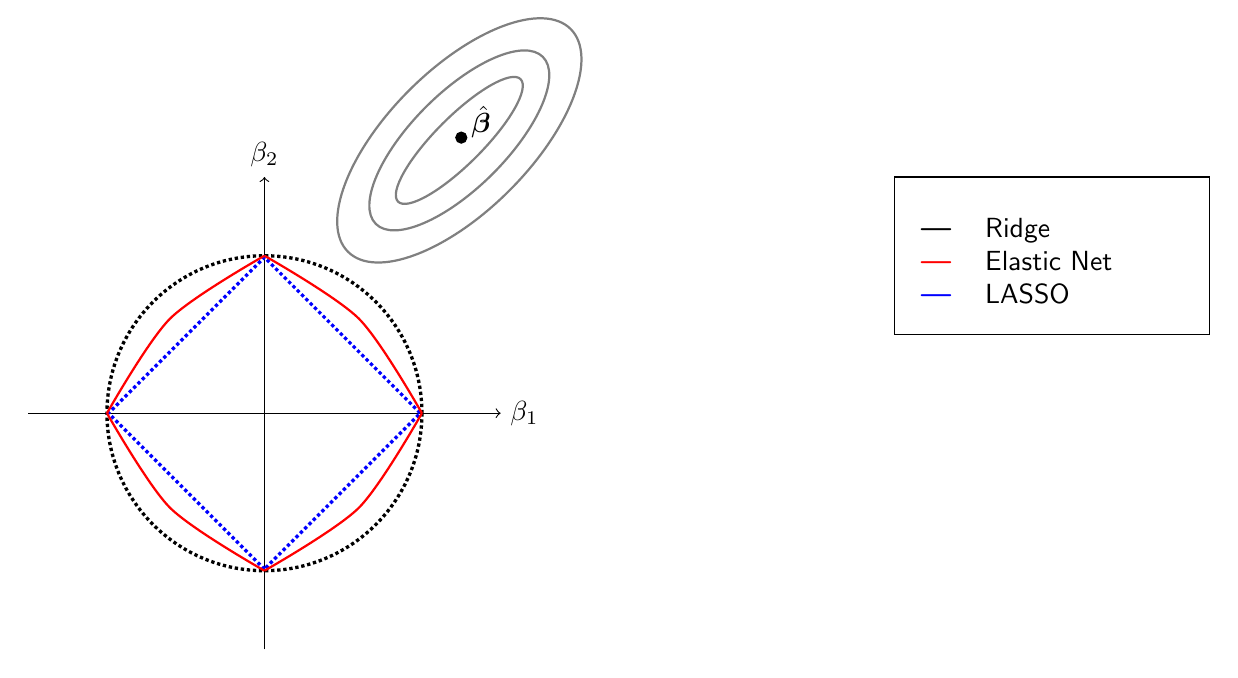
\begin{tikzpicture}
  % Set the axis range
  \def\xMin{-3}
  \def\xMax{3}
  \def\yMin{-3}
  \def\yMax{3}
  
  % Draw the axis
  \draw[->] (\xMin,0) -- (\xMax,0) node[right]{$\beta_1$};
  \draw[->] (0,\yMin) -- (0,\yMax) node[above] {$\beta_2$};
  
  % Plot the circumference
  \draw[line width=1.2pt, black, densely dotted] (0,0) circle[radius=2];
  
  % Plot the rotated square
  \draw[line width=1.2pt, blue, densely dotted, rotate around={45:(0,0)}] (-1.4,-1.4) rectangle (1.4,1.4);
  
  % Draw smooth curves
  \draw[red, thick, smooth] plot coordinates {(-2,0) (-1.2,1.2) (0,2)};
  \draw[red, thick, smooth] plot coordinates {(-2,0) (-1.2,-1.2) (0,-2)};
  \draw[red, thick, smooth] plot coordinates {(2,0) (1.2,1.2) (0,2)};
  \draw[red, thick, smooth] plot coordinates {(2,0) (1.2,-1.2) (0,-2)};

  % Draw the 45-degree ellipse outside the graph
  \draw[gray, thick, rotate around={45:(0,0)}] (4.2,0.7) ellipse (2 and 0.9);
  \draw[gray, thick, rotate around={45:(0,0)}] (4.2,0.7) ellipse (1.5 and 0.6);
  \draw[gray, thick, rotate around={45:(0,0)}] (4.2,0.7) ellipse (1.1 and 0.3);

  % Draw a dot inside the ellipse
  \filldraw[black] (2.5,3.5) circle (2pt);
  
  % Add the symbol \hat{\beta} at the center
  \node[black] at (2.75,3.7) {$\hat{\bm{\beta}}$};

  % Add legend
  \draw (8,3) -- (12,3) -- (12,1) -- (8,1) -- cycle;
  
  \node[anchor=west] at (8,1.9) {
    \begin{tabular}{l l}
      \textcolor{black}{\textbf{---}} & Ridge \\
      \textcolor{red}{\textbf{---}} & Elastic Net \\
      \textcolor{blue}{\textbf{---}} & LASSO \\
    \end{tabular}
  };

\end{tikzpicture}
\caption{Regularization Methods for Linear Regression}
  %\label{fig:reg_methods}
\end{figure}

The penalties from Figure 1 are particular cases of $L^p$-norms. For $p \geq 1$, the $L^p$-norm of $\bm{x} = (x_1,...,x_n)$ is:
$$||\bm{x}||_p = (|x_1|^p + |x_2|^p +...+|x_n|^p)^{\frac{1}{p}}$$

\textbf{I)} \textit{LASSO}

The Least Absolute Shrinkage and Selection Operator (Tibshirani, \citeyear{tibshirani1996regression}) is able to shrink coefficients up to zero and for this reason it is commonly used to select variables. Its penalty assumes the format of the $L^1$-norm. 
\begin{equation*}
    \bm{\hat{\beta}}_{\text{LASSO}}(\lambda) = \arg \min_{\bm{\beta} \in R^p}  ||\bm{y}-\bm{X \beta}||_2^2 + \lambda ||\bm{\beta}||_1
\end{equation*}  


\textbf{II)} \textit{Ridge}

The ridge regression (Hoerl;
Kennard, \citeyear{ridge}) is another method that implements shrinkage of the coefficients' values. However, unlike the LASSO, the ridge regression is not able to implement variable selection. This happens because its \textit{shrinkage penalty} assumes the format of a $L^2$-norm.
\begin{equation*}
    \bm{\hat{\beta}}_{\text{ridge}}(\lambda) = \arg \min_{\bm{\beta} \in R^p}  ||\bm{y}-\bm{X \beta}||_2^2 + \lambda ||\bm{\beta}||_2
\end{equation*}  

\textbf{III)} \textit{Elastic Net}

The elastic net (Zou; Hastie, \citeyear{elnet}) rests in between the LASSO and ridge. It tends to shrink the values of the coefficients more than the ridge but it cannot make them go to zero like the LASSO can. Its penalty is a mix of $L^1$ and $L^2$ norms:
\begin{equation*}
    \bm{\hat{\beta}}_{\text{elnet}}(\lambda_1, \lambda_2) = \arg \min_{\bm{\beta} \in R^p}  ||\bm{y}-\bm{X \beta}||_2^2 + \lambda_1 ||\bm{\beta}||_1 + \lambda_2 ||\bm{\beta}||_2
\end{equation*}  

\textbf{IV)} \textit{adaLASSO}

The adaptive LASSO (Zou, \citeyear{adalasso}) is an extension of the LASSO that presents theoretical advantages when compared to LASSO. In particular, the conditions for consistency of its variable selection are weaker than the conditions for the LASSO selection. The adaLASSO incorporates individual weights for each parameter, unlike LASSO which applies the same weighting to all parameters in the penalty. Irrelevant regressors should receive larger weights. To determine the values of the weights, we first compute $\bm{\hat{\beta}}_{\text{LASSO}}$ and then we define the weights:
$$w_j = \frac{1}{|\hat{\beta}_{\text{LASSO}_j}| + \frac{1}{\sqrt{n}}}, \text{ } j=1,...,p $$

\begin{equation*}
    \bm{\hat{\beta}}_{\text{adaLASSO}}(\lambda) = \arg \min_{\bm{\beta} \in R^p}  ||\bm{y}-\bm{X \beta}||_2^2 + \lambda \sum_{j=1}^p w_j |\beta_j|
\end{equation*}  

\subsection{Random Forest}

\hspace{1em} The random forest (Breiman, \citeyear{breiman2001random}) is a non-parametric method which applies bootstrap to regression trees, that allows to deal with non-linearity. Therefore, to explain the random forest we need to explain what a regression tree is.  

Suppose we have a dataset with $N$ observations and $K+1$ variables $x^1,...,x^K, \pi$, with $\pi$ being the target variable and $\bm{x}$ being the predictors. Fix $N^* < N$. A decision tree analyses the first $N^*$ observations of the variables, providing a tree $T^*(.)$ which is a decision rule to forecast the target variable. For instance, the predicted value of $\pi_{N^*+1}$ is: $$\hat{\pi}_{N^*+1} = T^*(x^1_{N^*+1},\hdots,x^K_{N^*+1})$$


%Let $N$ be the number of lines of the data we use to fit our models. A decision tree analyses all the $K$ columns and $N$ observations and it provides a tree $T^*(.)$ which is a decision rule to forecast $\pi_{N+1}$: $$\hat{\pi}_{N+1} = T^*(x^1_{N+1},\hdots,x^K_{N+1})$$

Figure 2 illustrates a decision tree where $\pi_i, \text{ }i=1,...,N^*$ represents the inflation at line $i$, and  $x^j = x^j_{N^*+1}$, and $c_i$ is a threshold for the decision rule. In this particular example, we presume that $\pi_i\neq \pi_j, \forall i \neq j$. Finally, notice that in our example the number of thresholds is equal to the number of observations ($N^*$), however in the majority of the cases the dependent variable can be explained with much fewer thresholds.

\definecolor{mediumspringgreen}{rgb}{0.0, 0.98, 0.6}
\definecolor{paleblue}{rgb}{0.69, 0.93, 0.93}
\definecolor{deepsaffron}{rgb}{1.0, 0.6, 0.2}
\definecolor{orange(webcolor)}{rgb}{1.0, 0.65, 0.0}
\definecolor{pastelyellow}{rgb}{0.99, 0.99, 0.59}
\definecolor{neonorange}{rgb}{2.55, 1.33, 0.58}
\definecolor{neoncarrot}{rgb}{1.0, 0.64, 0.26}
\definecolor{daffodil}{rgb}{1.0, 1.0, 0.19}

\begin{figure}[h]
    \centering
    \resizebox{8cm}{7cm}{%
    \begin{tikzpicture}[node distance={15mm}, thick, main/.style={draw, circle}]
  \node[main,fill=daffodil] (1) {$x^1 \leq c_1$};
  
  \node[main,fill=daffodil] (2) [below right=1cm and 1cm of 1] {$x^1 \leq c_2$};
  \node[main, fill=mediumspringgreen] (3) [below left=1cm and 1cm of 1] {$\pi_1$};

  
  \node[main,fill=daffodil] (4) [below right=1cm and 1cm of 2] {$x^2 \leq c_3$};
  \node[main,fill=mediumspringgreen] (5) [below left=1cm and 1cm of 2] {$\pi_2$};
  

  \node[main,fill=daffodil] (6) [below right=1.5cm and 1.5cm of 4] {$x^{K-1} \leq c_{N^*}$};
  \node[main,fill=mediumspringgreen] (7) [below left=1cm and 1cm of 4] {$\pi_3$};

  \node[main,fill=mediumspringgreen] (8) [below left=1cm and 1cm of 6] {$\pi_{N^*-1}$};
  \node[main,fill=mediumspringgreen] (9) [below right=1cm and 1cm of 6] {$\pi_{N^*}$};

  \draw[->] (1)-- (2);
  \draw[->] (1) -- (3);

  \draw[->] (2)-- (4);
  \draw[->] (2)-- (5);

  \draw[line width=1.8pt,loosely dotted] (4)-- (6);
  \draw[->] (4) -- (7);

  \draw[->] (6)--(8);
  \draw[->] (6)--(9);
  

\end{tikzpicture}
}
\caption{Illustration of a Regression Tree}
\end{figure}
    

The random forest applies bootstrap to regression trees. It generates many regression trees by randomly selecting some variables and some observations. The goal is to generate regression trees which are considerably different from each other. Finally, we take the average of the output of the regression trees. Let $B$ be the total number of trees. The random forest prediction is given by:

$$ \frac{1}{B} \sum_{b=1}^B \textit{T}^{*}_b(\textbf{X})$$

\hspace{-1.7em} where $\textit{T}^{*}_1$ is the first bootstrap regression tree, $\textit{T}^{*}_2$ is the second, and so on and so forth.   


\section{Error Measures}

\hspace{1em} To measure the performance of our forecasts, we compare the models from three statistics: root mean squared error (RMSE), mean absolute error (MAE), and median absolute deviation from the median (MAD):

$$RMSE_m = \sqrt{\frac{1}{T-T_0+1} \sum_{t=T_0}^T \hat{e}_{t,m}^2} $$

$$MAE_m = \frac{1}{T-T_0+1} \sum_{t=T_0}^T |\hat{e}_{t,m}|$$

$$MAD_m = \textnormal{median} \bigl\lvert \hat{e}_{t,m} - \textnormal{median}(\hat{e}_{t,m}) \bigr\rvert  $$

%The forecast error from model $m$ at time $t$ is given by:
%$$\hat{e}_{t,m} = \pi_t^{12} - %\hat{\pi}_{t|t-12,m}^{12}$$

\hspace{-1.7em} where $\hat{e}_{t,m}$ is the forecast error from model $m$ at time $t$ given by $\hat{e}_{t,m} = \pi_t^{12} - \hat{\pi}_{t|t-12,m}^{12}$. 

Given we make forecasts from 2014 until 2023, the value of the error measures of each model in this period can only explain how well each model behaved throughout this long window. Therefore, it does not evaluate how each model behaved during specific periods within the window. For this reason, we also compute the rolling RMSE of each model where each window has 12 months.
 

\chapter{Results}

\hspace{1em} We forecast Brazilian yearly inflation from January 2014 until January  2023, which means a total of 109 predictions. To compare the performance of each model with respect to the main benchmark, the median of the Focus survey, we normalize the values of their error measures by the values of the error measures from Focus. Initially, we analyse the values of the normalized error measures throughout the entire period of predictions. In a second moment, we compute RMSEs from 12-month rolling windows to have a dynamic view of the performance of models. We repeat this procedure for rolling and expanding windows forecasts. In this chapter, we are going to expose the results from the rolling window forecasts. The expanding window results can be found in \hyperref[sec:appendix.expanding]{Appendix C}.

Table 1 shows the values of the error measures from the rolling window forecasts normalized by the Focus RMSE (2.9) and MAE (2.1). When the normalized values are smaller than 1, the model outperform the Focus consensus. Finally, normalized RMSE and MAE from the random walk (RW) are 1.13 and 1.23, respectively, showing that the RW is outperformed by the main benchmark.


\begin{table}[h] \centering 
  \caption{RMSE, MAE and MAD for rolling window forecasts} 
  \label{rmserolling} 
    \resizebox{1.1\textwidth}{!}{
\begin{tabular}{@{\extracolsep{5pt}} ccccccccccccc} 
\\[-1.8ex]
\hline 
\hline 
\\[-1.8ex] 
\multicolumn{13}{c}{\textbf{Datasets:} $\bm{X^h,\text{ }h=1,...,12}$}\\ 
\midrule 
RMSE/(MAE)/ & 1 & 2 & 3 & 4 & 5 & 6 & 7 & 8 & 9 & 10 & 11 & 12 \\ 
\{MAD\} & & & & & & & & & & & & \\
\hline \\[-1.8ex] 
\textbf{RF} & \cellcolor{green!25}$0.42$ & $0.62$ & $0.60$ & $0.59$ & $0.60$ & $0.61$ & $0.58$ & $0.56$ & $0.56$ & $0.52$ & $0.52$ & $0.49$ \\ 
 & \cellcolor{blue!25}($0.49$) & ($0.70$) & ($0.68$) & ($0.68$) & ($0.68$) & ($0.68$) & ($0.66$) & ($0.63$) & ($0.63$) & ($0.59$) & ($0.58$) & ($0.53$) \\ 
 & \cellcolor{orange!25}\{$0.56$\} & \{$0.85$\} & \{$0.77$\} & \{$0.78$\} & \{$0.85$\} & \{$0.84$\} & \{$0.82$\} & \{$0.76$\} & \{$0.71$\} & \{$0.70$\} & \{$0.68$\} & \{$0.61$\} \\ 
\midrule
 
\textbf{CSR} & $0.65$ & $0.74$ & $0.72$ & $0.70$ & $1.51$ & $1.49$ & $1.26$ & $0.63$ & $0.61$ & $0.60$ & \cellcolor{green!25}$0.59$ & $0.72$ \\ 
  & ($0.72$) & ($0.84$) & ($0.80$) & ($0.78$) & ($0.91$) & ($0.90$) & ($0.86$) & ($0.71$) & ($0.70$) & ($0.69$) & \cellcolor{blue!25}($0.68$) & ($0.71$) \\ 
   & \{$0.78$\} & \{$1.01$\} & \{$0.94$\} & \{$0.86$\} & \{$0.88$\} & \{$0.90$\} & \{$0.93$\} & \{$0.93$\} & \{$0.89$\} & \{$0.80$\} & \cellcolor{orange!25}\{$0.74$\} & \{$0.76$\} \\ 
\midrule

\textbf{LASSO} & $0.44$ & $0.77$ & $2.39$ & $4.15$ & $4.60$ & $7$ & $1.22$ & $5.66$ & $1.99$ & \cellcolor{green!25}$0.43$ & $2.22$ & $1.67$ \\ 
  & ($0.46$) & ($0.85$) & ($1.18$) & ($1.42$) & ($1.28$) & ($1.46$) & ($0.65$) & ($1.31$) & ($0.72$) & \cellcolor{blue!25}($0.41$) & ($0.70$) & ($0.67$) \\
   & \{$0.51$\} & \{$0.96$\} & \{$0.84$\} & \{$0.74$\} & \{$0.50$\} & \{$0.48$\} & \{$0.47$\} & \{$0.50$\} & \{$0.47$\} & \{$0.41$\} & \{$0.44$\} & \cellcolor{orange!25}\{$0.40$\} \\ 
\midrule
  
\textbf{adaLASSO} & $0.45$ & $0.60$ & $1.63$ & $5.60$ & $4.37$ & $7.24$ & $1.14$ & $4.94$ & $0.51$ & \cellcolor{green!25}$0.35$ & $1.64$ & $0.46$ \\ 
  & ($0.49$) & ($0.68$) & ($1.06$) & ($1.57$) & ($1.22$) & ($1.48$) & ($0.62$) & ($1.15$) & ($0.45$) & \cellcolor{blue!25}($0.38$) & ($0.61$) & ($0.46$) \\ 
   & \{$0.57$\} & \{$0.66$\} & \{$0.88$\} & \{$0.67$\} & \{$0.49$\} & \{$0.50$\} & \{$0.47$\} & \{$0.47$\} & \{$0.39$\} & \cellcolor{orange!25}\{$0.38$\} & \{$0.45$\} & \{$0.43$\} \\
\midrule
  
\textbf{ElNet} & $0.45$ & $3.23$ & $2.35$ & $4.13$ & $4.50$ & $7.12$ & $1.22$ & $5.46$ & $2.39$ & $0.51$ & $2.68$ & \cellcolor{green!25}$0.44$ \\ 
  & ($0.50$) & ($1.25$) & ($1.20$) & ($1.40$) & ($1.28$) & ($1.46$) & ($0.67$) & ($1.29$) & ($0.80$) & ($0.45$) & ($0.77$) & \cellcolor{blue!25}($0.45$) \\ 
   & \{$0.48$\} & \{$0.96$\} & \{$0.92$\} & \{$0.78$\} & \{$0.56$\} & \{$0.51$\} & \{$0.45$\} & \{$0.50$\} & \{$0.47$\} & \{$0.48$\} & \{$0.43$\} & \cellcolor{orange!25}\{$0.39$\} \\ 
\midrule
\textbf{Ridge} & $0.52$ & $1.04$ & $1.88$ & $4.05$ & $4.81$ & $5.32$ & $1.90$ & $3.82$ & $3.69$ & $1.40$ & $1.76$ & \cellcolor{green!25}$0.51$ \\ 
  & ($0.57$) & ($1.24$) & ($1.32$) & ($1.43$) & ($1.27$) & ($1.27$) & ($0.89$) & ($1.14$) & ($0.98$) & ($0.57$) & ($0.67$) & \cellcolor{blue!25}($0.47$) \\ 
   & \{$0.58$\} & \{$1.66$\} & \{$1.15$\} & \{$0.92$\} & \{$0.69$\} & \{$0.54$\} & \{$0.51$\} & \{$0.48$\} & \{$0.48$\} & \{$0.43$\} & \{$0.45$\} & \cellcolor{orange!25}\{$0.35$\} \\
\hline \\[-1.8ex] 
\end{tabular} 
}
\resizebox{1.1\textwidth}{!}{
\begin{minipage}{16.4cm}
    \hline
    \hline
    \vspace{0.1cm}
    \small The columns represent the datasets. The coloured values correspond to the best result of the models for each error measure. 

        
    \end{minipage}
    }
\end{table} 


The random forest consistently beats the benchmark across all datasets and the gains can be as large as $58\%$ in terms of RMSE. The CSR also beats the benchmark with multiple datasets but unlike the random forest, sometimes it is beaten by the Focus. The shrinkage methods exhibit significant heterogeneity across datasets. For instance, when data is accumulated from 3 to 8 months, the shrinkage methods consistently fail to beat the benchmark. On the other hand, they show significant gains in comparison to the Focus consensus when data is not accumulated or accumulated in 12 months.

In general, the six models consistently outperform the benchmark when data is not accumulated or accumulated in 12 months. However, the overall performance of the models varies across the other datasets. For this reason, our analysis emphasizes the results obtained with these two datasets.

When regressors are not accumulated, all the models outperform the benchmark showing gains around 50\% in terms of RMSE. In particular, the random forest achieves the best result.

When regressors are accumulated in 12 months, all the models (except for LASSO) show significant gains in terms of RMSE (up to 56\%) when compared to the Focus. This result seems reasonable given that we are forecasting a variable that is also accumulated in 12 months. The operation of accumulating the regressors in 12 months should make them smoother and this could be an interesting property when forecasting a yearly variable.

%On the other hand, the the majority of the models presented even larger gains when regressors were not accumulated. Therefore, we conclude that in the case of rolling window forecasts, there were no gains from accumulating the explanatory variables. 

Table 2 shows descriptive statistics about the performance of models across all datasets. RF and CSR are the only models with an average RMSE smaller than the benchmark. This result is expected given that in Table 1 we see these two models consistently beating the benchmark across multiple datasets. Finally, we find that adaLASSO obtains at the same time the lowest and the highest RMSE and MAE across our datasets. Similarly, ridge shows at the same time the lowest and the highest MAD. These two results are in line with our previous finding that shrinkage methods performance varies markedly across different datasets.  

\begin{table}[h] \centering 
  \caption{Descriptive statistics: rolling window forecasts errors} 
  \label{} 
  \resizebox{1.1\textwidth}{!}{
\begin{tabular}{@{\extracolsep{5pt}} cccccccccc} 
\\[-1.8ex]\hline 
\hline \\[-1.8ex] 
 & $\overline{\text{RMSE}}$ & $\overline{\text{MAE}}$ & $\overline{\text{MAD}}$ & $\textbf{max}_{\text{RMSE}}$ & $\textbf{max}_{\text{MAE}}$ & $\textbf{max}_{\text{MAD}}$ & $\textbf{min}_{\text{RMSE}}$ & $\textbf{min}_{\text{MAE}}$ & $\textbf{min}_{\text{MAD}}$ \\ 
\hline \\[-1.8ex] 
\textbf{RF} & \cellcolor{green!25}$0.56$ & \cellcolor{green!25}$0.63$ & $0.74$ & $0.62$ & $0.70$ & $0.85$ & $0.42$ & $0.49$ & $0.56$ \\ 
\textbf{CSR} & $0.85$ & $0.77$ & $0.87$ & $1.51$ & $0.91$ & $1.01$ & $0.59$ & $0.68$ & $0.74$ \\ 
\textbf{LASSO} & $2.71$ & $0.92$ & $0.56$ & $7.00$ & $1.46$ & $0.96$ & $0.43$ & $0.41$ & $0.40$ \\ 
\textbf{adaLASSO} & $2.41$ & $0.85$ & \cellcolor{green!25}$0.53$ & $7.24$ & $1.57$ & $0.88$ & \cellcolor{green!25}$0.35$ & \cellcolor{green!25}$0.38$ & $0.38$ \\ 
\textbf{ElNet} & $2.87$ & $0.96$ & $0.58$ & $7.12$ & $1.46$ & $0.96$ & $0.44$ & $0.45$ & $0.39$ \\ 
\textbf{Ridge} & $2.56$ & $0.98$ & $0.69$ & $5.32$ & $1.43$ & $1.66$ & $0.51$ & $0.47$ & \cellcolor{green!25}$0.35$ \\ 
\textbf{RW} & $1.13$ & $1.23$ & $1.04$ & $1.13$ & $1.23$ & $1.04$ & $1.13$ & $1.23$ & $1.04$ \\ 
\hline \\[-1.8ex] 
\end{tabular} 
}
\end{table}

Medeiros et al. (\citeyear{datarich}) showed that ML models (especially the RF) outperformed traditional times-series univariate models in forecasting US inflation, mainly during volatile periods. We expect Brazilian inflation to be more volatile in comparison to the US given that "emerging markets usually exhibit higher and more volatile inflation" (Garcia; Medeiros; Vasconcelos, \citeyear{RealTime}). For this reason, Brazilian data should be an interesting resource to test machine learning methods (high) performance when inflation is more volatile.

Our 12-month rolling RMSE computations start in January 2015 and end in January 2023. In Figure 3, we can see that from 2015 until the beginning of 2017 and from 2021 onward the majority of the ML models beat the Focus. This is expected given that these are two periods when Brazilian inflation grew more than it normally does. In the first period, the growth of inflation is related to the government's intervention in energy prices and, more recently, is related to the Covid. Notice that even though the pandemic starts in March 2020, it only completely impacts the 12-month accumulated inflation from February 2021 onward. 


\begin{figure}[htbp]
    \centering
    \resizebox{\textwidth}{!}{\includegraphics{error_1_3_6_12.pdf}}
    \caption{Rolling RMSE}
    \label{fig:error}
\end{figure}

These plots illustrate a similar result to that shown in Table 1: in general, the models are more accurate when we do not accumulate the data or accumulate it in 12 months. With these two datasets, the only period of time when the models are generally outperformed by the Focus is from February 2019 to February 2021. However, when we use the other datasets, the group of models presents more heterogeneous results through time. In addition, we get bigger and more volatile errors through time when we use these other datasets. The complete version of the plots can be found in the \hyperref[sec:appendix.error.rolling]{\textcolor{blue}{Appendix B}}. 

A desired property for a statistical model is the ability of beating a benchmark as many times as possible. Table 3 shows the percentage of the times when the rolling RMSE of each model-dataset pair is smaller than the rolling RMSE of the Focus. The total number of 12-month rolling RMSEs computed from January 2015 to January 2023 is 97. We show that for 
all the models, the best results are either obtained when data is not accumulated or accumulated in 12 months. In particular, the RF with non-accumulated regressors beats the FOCUS more than 80\% of the time.

\begin{table}[h] \centering 
  \caption{Percentage of the times when the models beat Focus} 
  \label{} 
    \resizebox{1.1\textwidth}{!}{
\begin{tabular}{@{\extracolsep{5pt}} ccccccccccccc} 
\\[-1.8ex]\hline 
\hline \\[-1.8ex] 
 & 1 & 2 & 3 & 4 & 5 & 6 & 7 & 8 & 9 & 10 & 11 & 12 \\ 
\hline \\[-1.8ex] 
\textbf{RF} & \cellcolor{green!25}$80.41$ & $53.61$ & $58.76$ & $59.79$ & $67.01$ & $68.04$ & $70.10$ & $75.26$ & $76.29$ & $75.26$ & $76.29$ & $70.10$ \\ 
\textbf{CSR} & $62.89$ & $45.36$ & $48.45$ & $48.45$ & $44.33$ & $43.30$ & $45.36$ & $54.64$ & $55.67$ & $58.76$ & $60.82$ & \cellcolor{green!25}$69.07$ \\ 
\textbf{LASSO} & \cellcolor{green!25}$73.20$ & $54.64$ & $32.99$ & $41.24$ & $49.48$ & $58.76$ & $65.98$ & $43.30$ & $55.67$ & $73.20$ & $73.20$ & $64.95$ \\ 
\textbf{adaLASSO} & \cellcolor{green!25}$75.26$ & $60.82$ & $36.08$ & $43.30$ & $45.36$ & $53.61$ & $67.01$ & $56.70$ & $76.29$ & $75.26$ & $70.10$ & $75.26$ \\ 
\textbf{ElNet} & $74.23$ & $40.21$ & $31.96$ & $39.18$ & $46.39$ & $58.76$ & $55.67$ & $43.30$ & $53.61$ & $75.26$ & $74.23$ & \cellcolor{green!25}$77.32$ \\ 
\textbf{Ridge} & $60.82$ & $28.87$ & $16.49$ & $31.96$ & $45.36$ & $47.42$ & $40.21$ & $35.05$ & $58.76$ & $68.04$ & $67.01$ & \cellcolor{green!25}$76.29$ \\ 
\hline \\[-1.8ex] 
\end{tabular} 
}
\resizebox{1.1\textwidth}{!}{
\begin{minipage}{16.4cm}
    \hline
    \hline
    \vspace{0.1cm}
    \small Percentage of times that 12-month rolling RMSE of a model-dataset pair is smaller than the 12-month rolling RMSE of the Focus consensus. RW beats the benchmark only about 30\% of the time.
    \end{minipage}
    }
\end{table} 

Finally, the results from the expanding window forecasts are similar to the results from the rolling window forecasts. One remarkable difference is that when using expanding window, all the models (except for the RF) obtain the best MAD when data is accumulated in 12 months.


\chapter{Conclusion}

\hspace{1em} We investigate the performance of six machine learning methods for forecasting 12-month-ahead yearly inflation, considering the Brazilian case. In particular, we study whether there are gains from accumulating the regressors in 1 to 12 months. Our benchmark is the median of the Focus survey of inflation expectations. 

Our main findings are:

\begin{enumerate}
    \item Machine learning models consistently outperform the Focus consensus when data is not accumulated or it is accumulated in 12 months. 

    \item Machine learning models (especially RF) consistently outperform the Focus during periods of more volatile inflation.

    \item The random forest (RF) is the only model that outperforms the benchmark in every dataset. In particular, the best model is the RF without accumulating regressors.

    \item The performance of shrinkage methods varies considerably across different datasets. 
    
\end{enumerate}

Following our first finding, we recommend evaluating forecasts when regressors are accumulated in 12 months as a robustness exercise after computing the forecasts without applying transformations to the regressors.




\bibliography{references}

\appendix






\chapter{Table of transformations}
\label{sec:transformation.table}

\hspace{1em} The table provides the classification, the code (from the \href{https://www3.bcb.gov.br/sgspub/localizarseries/localizarSeries.do?method=prepararTelaLocalizarSeries}{Time Series Management System}), the frequency, the unity of measure, the lags, and finally the transformation applied to each predictor. When Transformation=0, the variable is not transformed. Transformations 1, 2, and 3 are explained \hyperref[sec:transformations]{here}.

\begin{table}[!htbp] \centering 
  %\caption{} 
  %\label{} 
  \resizebox{1.1\textwidth}{!}{
\begin{tabular}{@{\extracolsep{5pt}} cccccccc} 
\\[-1.8ex]\hline 
\hline \\[-1.8ex] 
 & Group & Variable & Code & Frequency & Unity & Transformation & Lag \\ 
\hline \\[-1.8ex] 
1 & PRICES & ipca & 433 & M & month\_\%\_var & 2 & 1 \\ 
2 & PRICES & ipca\_ali & 1635 & M & month\_\%\_var & 2 & 1 \\ 
3 & PRICES & ipca\_hab & 1636 & M & month\_\%\_var & 2 & 1 \\ 
4 & PRICES & ipca\_resid & 1637 & M & month\_\%\_var & 2 & 1 \\ 
5 & PRICES & ipca\_vest & 1638 & M & month\_\%\_var & 2 & 1 \\ 
6 & PRICES & ipca\_transp & 1639 & M & month\_\%\_var & 2 & 1 \\ 
7 & PRICES & ipca\_comunic & 1640 & M & month\_\%\_var & 2 & 1 \\ 
8 & PRICES & ipca\_saude & 1641 & M & month\_\%\_var & 2 & 1 \\ 
9 & PRICES & ipca\_desp & 1642 & M & month\_\%\_var & 2 & 1 \\ 
10 & PRICES & ipca\_educ & 1643 & M & month\_\%\_var & 2 & 1 \\ 
11 & PRICES & ipc\_BR & 191 & M & month\_\%\_var & 2 & 1 \\ 
12 & PRICES & igp\_M & 189 & M & month\_\%\_var & 2 & 1 \\ 
13 & PRICES & igp\_DI & 190 & M & month\_\%\_var & 2 & 1 \\ 
14 & PRICES & igp10 & 7447 & M & month\_\%\_var & 2 & 1 \\ 
15 & PRICES & ipca15 & 7478 & M & month\_\%\_var & 2 & 1 \\ 
16 & PRICES & bm\_broad & 1788 & M & cmu\_thousand & 1 & 2 \\ 
17 & PRICES & bm & 1785 & M & cmu\_thousand & 1 & 2 \\ 
18 & PRICES & m1 & 1783 & M & cmu\_thousand & 1 & 2 \\ 
19 & PRICES & m2 & 1786 & M & cmu\_thousand & 1 & 2 \\ 
20 & PRICES & m3 & 27813 & M & cmu\_thousand & 1 & 2 \\ 
21 & PRICES & m4 & 27815 & M & cmu\_thousand & 1 & 2 \\
\hline \\[-1.8ex]
22 & COMMODITIES & icbr & 27574 & M & index & 1 & 1 \\ 
23 & COMMODITIES & icbr\_agr & 27575 & M & index & 1 & 1 \\ 
24 & COMMODITIES & icbr\_metal & 27576 & M & index & 1 & 1 \\ 
25 & COMMODITIES & icbr\_energy & 27577 & M & index & 1 & 1 \\ 
\hline \\[-1.8ex]
26 & ACTIVITY & ibcbr & 24363 & M & index & 1 & 3 \\ 
27 & ACTIVITY & pimpf & 21859 & M & index & 1 & 2 \\ 
28 & ACTIVITY & pimpf\_extract & 21861 & M & index & 1 & 2 \\ 
29 & ACTIVITY & pimpf\_manufac & 21862 & M & index & 1 & 2 \\ 
30 & ACTIVITY & retail\_total & 1455 & M & index & 1 & 2 \\ 
31 & ACTIVITY & retail\_fuel & 1483 & M & index & 1 & 2 \\ 
32 & ACTIVITY & retail\_supermarket & 1496 & M & index & 1 & 2 \\ 
33 & ACTIVITY & retail\_clothing & 1509 & M & index & 1 & 2 \\ 
34 & ACTIVITY & retail\_house & 1522 & M & index & 1 & 2 \\ 
35 & ACTIVITY & retail\_drugstore & 20099 & M & index & 1 & 2 \\ 
36 & ACTIVITY & retail\_paper & 20101 & M & index & 1 & 2 \\ 
\hline \\[-1.8ex] 
\end{tabular} 
}
\end{table}



\begin{table}[!htbp] \centering 
  %\caption{} 
  %\label{} 
  \resizebox{1.1\textwidth}{!}{
\begin{tabular}{@{\extracolsep{5pt}} cccccccc} 
\\[-1.8ex]\hline 
\hline \\[-1.8ex] 
 & Group & Variable & Code & Frequency & Unity & Transformation & Lag \\
\hline \\[-1.8ex] 
37 & ACTIVITY & retail\_office & 20102 & M & index & 1 & 2 \\ 
38 & ACTIVITY & retail\_others & 20104 & M & index & 1 & 2 \\ 
39 & ACTIVITY & retail\_building & 20105 & M & index & 1 & 2 \\ 
40 & ACTIVITY & retail\_auto & 1548 & M & index & 1 & 2 \\ 
41 & ACTIVITY & prod\_vehicles & 1373 & M & units & 1 & 1 \\ 
42 & ACTIVITY & prod\_agr\_mach & 1388 & M & units & 1 & 1 \\ 
43 & ACTIVITY & vehicle\_sales & 7389 & M & barrels\_day\_thousand & 1 & 1 \\ 
44 & ACTIVITY & tcu & 24352 & M & \% & 3 & 1 \\ 
\hline \\[-1.8ex] 
45 & EMPLOYMENT & min\_wage & 1619 & M & cmu & 1 & 2 \\ 
46 & EMPLOYMENT & aggreg\_wage & 10790 & M & R\$ & 1 & 0 \\ 
47 & EMPLOYMENT & unem & NA & M & \% & 3 & 3 \\ 
\hline \\[-1.8ex] 
48 & ELECTRICITY & elec & 1406 & M & GWh & 1 & 3 \\ 
49 & ELECTRICITY & elec\_com & 1402 & M & GWh & 1 & 3 \\ 
50 & ELECTRICITY & elec\_res & 1403 & M & GWh & 1 & 3 \\ 
51 & ELECTRICITY & elec\_ind & 1404 & M & GWh & 1 & 3 \\ 
\hline \\[-1.8ex]
52 & CONFIDENCE & cons\_confidence & 4393 & M & index & 1 & 1 \\ 
53 & CONFIDENCE & future\_expec & 4395 & M & index & 1 & 1 \\ 
\hline \\[-1.8ex]
54 & FINANCE & irf\_m & 12461 & D & index & 1 & 1 \\ 
55 & FINANCE & ima\_s & 12462 & D & index & 1 & 1 \\ 
56 & FINANCE & ima\_b & 12466 & D & index & 1 & 1 \\ 
57 & FINANCE & ima & 12469 & D & index & 1 & 1 \\ 
58 & FINANCE & saving\_deposits & 1838 & M & cmu\_thousand & 1 & 2 \\ 
59 & FINANCE & selic & 4390 & M & \%\_pm & 0 & 1 \\ 
60 & FINANCE & cdi & 4391 & M & \%\_pm & 0 & 1 \\ 
61 & FINANCE & tjlp & 256 & M & \%\_py & 0 & 1 \\ 
62 & FINANCE & ibovespa & NA & D & \%\_pm & 0 & 1 \\ 
\hline \\[-1.8ex]
63 & CREDIT & cred\_total & 28183 & M & R\$\_million & 1 & 2 \\ 
64 & CREDIT & cred\_gdp & 28215 & M & \% & 3 & 2 \\ 
65 & CREDIT & indebt\_house\_19882 & 19882 & M & \% & 3 & 4 \\ 
66 & CREDIT & indebt\_house\_20400 & 20400 & M & \% & 3 & 4 \\ 
\hline \\[-1.8ex]
67 & GOVERNMENT & net\_debt\_gdp & 4513 & M & \% & 3 & 2 \\ 
68 & GOVERNMENT & net\_debt & 4478 & M & R\$\_million & 3 & 2 \\ 
69 & GOVERNMENT & net\_debt\_fedgov\_bcb & 4468 & M & R\$\_million & 3 & 2 \\ 
70 & GOVERNMENT & net\_debt\_states & 4472 & M & R\$\_million & 3 & 2 \\ 
71 & GOVERNMENT & net\_debt\_cities & 4473 & M & R\$\_million & 3 & 2 \\ 
72 & GOVERNMENT & primary\_result & 4649 & M & R\$\_million & 3 & 2 \\ 
73 & GOVERNMENT & debt\_fedgov\_old & 4502 & M & R\$\_million & 1 & 2 \\ 
74 & GOVERNMENT & debt\_fedgov\_new & 13761 & M & R\$\_million & 1 & 2 \\ 
75 & GOVERNMENT & treasury\_emit & 4151 & M & cmu\_million & 1 & 2 \\ 
76 & GOVERNMENT & treasury\_mkt & 4154 & M & cmu\_million & 1 & 2 \\ 
77 & GOVERNMENT & treasury\_term & 10616 & M & months & 3 & 2 \\ 
78 & GOVERNMENT & treasury\_dur & 10617 & M & months & 3 & 2 \\ 
\hline \\[-1.8ex]
79 & INTERNATIONAL & reer & 11752 & M & index & 1 & 2 \\ 
80 & INTERNATIONAL & usd\_brl\_end & 3695 & M & cmu\_US\$ & 1 & 1 \\ 
81 & INTERNATIONAL & usd\_brl\_avg & 3697 & M & cmu\_US\$ & 1 & 1 \\ 
82 & INTERNATIONAL & current\_account & 22701 & M & US\$\_million & 1 & 2 \\ 
83 & INTERNATIONAL & trade\_balance & 22707 & M & US\$\_million & 1 & 2 \\ 
84 & INTERNATIONAL & imports & 22709 & M & US\$\_million & 1 & 2 \\ 


\hline \\[-1.8ex] 
\end{tabular} 
}
\end{table}










\chapter{Rolling window forecasts: rolling RMSE}\label{sec:appendix.error.rolling}

\begin{figure}[htbp]
    \centering
    \resizebox{\textwidth}{!}{\includegraphics{error_1_6.pdf}}
    %\caption{This is the figure caption.}
    \label{fig:error}
\end{figure}

\begin{figure}[htbp]
    \centering
    \resizebox{\textwidth}{!}{\includegraphics{error_7_12.pdf}}
    %\caption{This is the figure caption.}
    \label{fig:error}
\end{figure}



\chapter{Expanding Window Results}\label{sec:appendix.expanding}
\begin{table}[h] \centering 
  \caption{RMSE, MAE and MAD for expanding window forecasts} 
  \label{rmseexpanding} 
    \resizebox{1.1\textwidth}{!}{
\begin{tabular}{@{\extracolsep{5pt}} ccccccccccccc} 
\\[-1.8ex]\hline 
\hline \\[-1.8ex] 
\multicolumn{13}{c}{\textbf{Datasets:} $\bm{X^h,\text{ }h=1,...,12}$}\\ 
\midrule 
RMSE/(MAE)/ & 1 & 2 & 3 & 4 & 5 & 6 & 7 & 8 & 9 & 10 & 11 & 12 \\ 
\{MAD\} & & & & & & & & & & & & \\
\hline \\[-1.8ex] 
\textbf{RF} & \cellcolor{green!25}$0.45$ & $0.65$ & $0.62$ & $0.61$ & $0.60$ & $0.59$ & $0.59$ & $0.58$ & $0.57$ & $0.55$ & $0.53$ & $0.50$ \\ 
 & \cellcolor{blue!25}($0.50$) & ($0.76$) & ($0.73$) & ($0.70$) & ($0.68$) & ($0.66$) & ($0.66$) & ($0.65$) & ($0.63$) & ($0.62$) & ($0.59$) & ($0.54$) \\ 
 & \cellcolor{orange!25}\{$0.56$\} & \{$0.92$\} & \{$0.90$\} & \{$0.93$\} & \{$0.89$\} & \{$0.74$\} & \{$0.78$\} & \{$0.76$\} & \{$0.69$\} & \{$0.73$\} & \{$0.69$\} & \{$0.66$\} \\
\midrule 
 
\textbf{CSR} & $0.78$ & $0.76$ & $0.75$ & $0.75$ & $0.74$ & $0.74$ & $0.74$ & $0.73$ & $0.72$ & $0.71$ & \cellcolor{green!25}$0.69$ & $0.80$ \\ 
  & ($0.83$) & ($0.89$) & ($0.87$) & ($0.86$) & ($0.85$) & ($0.84$) & ($0.83$) & ($0.83$) & ($0.83$) & ($0.81$) & \cellcolor{blue!25}($0.79$) & ($0.86$) \\ 
 & \{$0.93$\} & \{$1.13$\} & \{$1.05$\} & \{$1.00$\} & \{$0.97$\} & \{$1.01$\} & \{$1.02$\} & \{$1.06$\} & \{$1.00$\} & \{$1.00$\} & \{$0.94$\} & \cellcolor{orange!25}\{$0.83$\} \\
\midrule 
  
\textbf{LASSO} & \cellcolor{green!25}$0.45$ & $0.66$ & $0.63$ & $0.62$ & $2.04$ & $0.51$ & $0.52$ & $1.56$ & $1.64$ & $1.65$ & $0.49$ & $2.31$ \\ 
  & ($0.50$) & ($0.77$) & ($0.73$) & ($0.73$) & ($0.92$) & ($0.57$) & ($0.54$) & ($0.72$) & ($0.69$) & ($0.64$) & \cellcolor{blue!25}($0.48$) & ($0.78$) \\ 
 & \{$0.51$\} & \{$1.04$\} & \{$0.89$\} & \{$0.76$\} & \{$0.77$\} & \{$0.65$\} & \{$0.61$\} & \{$0.48$\} & \{$0.49$\} & \{$0.40$\} & \{$0.50$\} & \cellcolor{orange!25}\{$0.39$\} \\
\midrule 
  
\textbf{adaLASSO} & $0.46$ & $0.59$ & $0.59$ & $0.59$ & $0.56$ & $0.50$ & $0.47$ & $0.64$ & $1.48$ & $1.64$ & \cellcolor{green!25}$0.42$ & $1.72$ \\ 
  & ($0.52$) & ($0.69$) & ($0.68$) & ($0.69$) & ($0.65$) & ($0.56$) & ($0.50$) & ($0.52$) & ($0.64$) & ($0.64$) & \cellcolor{blue!25}($0.45$) & ($0.70$) \\ 
 & $0.49$ & $0.90$ & $0.90$ & $0.83$ & $0.75$ & $0.67$ & $0.55$ & $0.51$ & $0.45$ & $0.43$ & $0.52$ & \cellcolor{orange!25}$0.41$ \\
\midrule 
  
\textbf{ElNet} & $0.48$ & $0.68$ & $0.64$ & $0.63$ & $0.64$ & $0.55$ & $0.53$ & $1.63$ & $1.33$ & $1.66$ & \cellcolor{green!25}$0.47$ & $2.28$ \\ 
  & ($0.54$) & ($0.79$) & ($0.74$) & ($0.73$) & ($0.69$) & ($0.60$) & ($0.56$) & ($0.73$) & ($0.64$) & ($0.64$) & \cellcolor{blue!25}($0.48$) & ($0.78$) \\ 
 & $0.53$ & $0.99$ & $0.89$ & $0.82$ & $0.77$ & $0.66$ & $0.64$ & $0.57$ & $0.53$ & $0.45$ & $0.49$ & \cellcolor{orange!25}$0.41$ \\
\midrule 
  
\textbf{Ridge} & \cellcolor{green!25}$0.58$ & $0.98$ & $0.98$ & $1.22$ & $1.86$ & $1.15$ & $0.92$ & $3.16$ & $2.88$ & $1.62$ & $1.01$ & $1.32$ \\ 
  & \cellcolor{blue!25}($0.63$) & ($1.17$) & ($1.17$) & ($1.16$) & ($1.01$) & ($0.82$) & ($0.74$) & ($1.07$) & ($0.96$) & ($0.68$) & ($0.66$) & ($0.67$) \\  
   & $0.59$ & $1.50$ & $1.50$ & $1.37$ & $0.92$ & $0.64$ & $0.65$ & $0.62$ & $0.56$ & $0.52$ & $0.54$ & \cellcolor{orange!25}$0.42$ \\
\hline \\[-1.8ex] 
\end{tabular} 
}
\resizebox{1.1\textwidth}{!}{
\begin{minipage}{16.4cm}
    \hline
    \hline
    \vspace{0.1cm}
    \small The columns represent the datasets. The coloured values correspond to the best result of the models for each error measure. 
    \end{minipage}
    }
\end{table} 











\begin{table}[h] \centering 
  \caption{Descriptive statistics: expanding window forecasts errors} 
  \label{} 
  \resizebox{1.1\textwidth}{!}{
\begin{tabular}{@{\extracolsep{5pt}} cccccccccc} 
\\[-1.8ex]\hline 
\hline \\[-1.8ex] 
 & $\overline{\text{RMSE}}$ & $\overline{\text{MAE}}$ & $\overline{\text{MAD}}$ & $\textbf{max}_{\text{RMSE}}$ & $\textbf{max}_{\text{MAE}}$ & $\textbf{max}_{\text{MAD}}$ & $\textbf{min}_{\text{RMSE}}$ & $\textbf{min}_{\text{MAE}}$ & $\textbf{min}_{\text{MAD}}$ \\ 
\hline \\[-1.8ex] 
\textbf{RF} & \cellcolor{green!25}$0.57$ & $0.64$ & $0.77$ & $0.65$ & $0.76$ & $0.93$ & $0.45$ & $0.50$ & $0.56$ \\ 
\textbf{CSR} & $0.74$ & $0.84$ & $0.99$ & $0.80$ & $0.89$ & $1.13$ & $0.69$ & $0.79$ & $0.83$ \\ 
\textbf{LASSO} & $1.09$ & $0.67$ & \cellcolor{green!25}$0.62$ & $2.31$ & $0.92$ & $1.04$ & $0.45$ & $0.48$ & \cellcolor{green!25}$0.39$ \\ 
\textbf{adaLASSO} & $0.81$ & \cellcolor{green!25}$0.60$ & \cellcolor{green!25}$0.62$ & $1.72$ & $0.70$ & $0.90$ & \cellcolor{green!25}$0.42$ & \cellcolor{green!25}$0.45$ & $0.41$ \\ 
\textbf{ElNet} & $0.96$ & $0.66$ & $0.64$ & $2.28$ & $0.79$ & $0.99$ & $0.47$ & $0.48$ & $0.41$ \\ 
\textbf{Ridge} & $1.47$ & $0.89$ & $0.82$ & $3.16$ & $1.17$ & $1.50$ & $0.58$ & $0.63$ & $0.42$ \\ 
\textbf{RW} & $1.13$ & $1.23$ & $1.04$ & $1.13$ & $1.23$ & $1.04$ & $1.13$ & $1.23$ & $1.04$ \\ 
\hline \\[-1.8ex] 
\end{tabular} 
}
\end{table}








\begin{table}[htpb] \centering 
  \caption{Percentage of the times when the models beat Focus} 
  \label{} 
    \resizebox{1.1\textwidth}{!}{
\begin{tabular}{@{\extracolsep{5pt}} ccccccccccccc} 
\\[-1.8ex]\hline 
\hline \\[-1.8ex] 
 & 1 & 2 & 3 & 4 & 5 & 6 & 7 & 8 & 9 & 10 & 11 & 12 \\ 
\hline \\[-1.8ex] 
\textbf{RF} & \cellcolor{green!25}$80.41$ & $53.61$ & $61.86$ & $68.04$ & $70.10$ & $73.20$ & $74.23$ & $73.20$ & $75.26$ & $74.23$ & $76.29$ & $70.10$ \\ 
\textbf{CSR} & $55.67$ & $41.24$ & $49.48$ & $50.52$ & $51.55$ & $49.48$ & $49.48$ & $50.52$ & $52.58$ & $55.67$ & $56.70$ & \cellcolor{green!25}$65.98$ \\ 
\textbf{LASSO} & $73.20$ & $65.98$ & $64.95$ & $67.01$ & $57.73$ & $74.23$ & \cellcolor{green!25}$75.26$ & $50.52$ & $62.89$ & $69.07$ & $71.13$ & $62.89$ \\ 
\textbf{adaLASSO} & $74.23$ & $72.16$ & $72.16$ & $70.10$ & $73.20$ & $74.23$ & \cellcolor{green!25}$78.35$ & $77.32$ & $62.89$ & $69.07$ & $75.26$ & $62.89$ \\ 
\textbf{ElNet} & $72.16$ & $59.79$ & $60.82$ & $64.95$ & $71.13$ & \cellcolor{green!25}$74.23$ & $69.07$ & $62.89$ & $65.98$ & $71.13$ & $73.20$ & $61.86$ \\ 
\textbf{Ridge} & \cellcolor{green!25}$61.86$ & $25.77$ & $25.77$ & $13.40$ & $37.11$ & $43.30$ & $46.39$ & $47.42$ & $51.55$ & \cellcolor{green!25}$61.86$ & $57.73$ & \cellcolor{green!25}$61.86$ \\ 
\hline \\[-1.8ex] 
\end{tabular} 
}
    \resizebox{1.1\textwidth}{!}{
\begin{minipage}{16.4cm}
    \hline
    \hline
    \vspace{0.1cm}
    \small Percentage of times that 12-month rolling RMSE of a model-dataset pair is smaller than the 12-month rolling RMSE of the Focus consensus. RW beats the benchmark only about 30\% of the time.

    \end{minipage}
    }
\end{table} 


\newpage

\begin{figure}[htbp]
    \centering
    \resizebox{\textwidth}{!}{\includegraphics{error_exp_1_6.pdf}}
    %\caption{This is the figure caption.}
    \label{fig:error}
\end{figure}

\begin{figure}[htbp]
    \centering
    \resizebox{\textwidth}{!}{\includegraphics{error_exp_7_12.pdf}}
    %\caption{This is the figure caption.}
    \label{fig:error}
\end{figure}


\end{document}

